\documentclass[pdftex,letterpaper,10pt]{article}
\usepackage[pdftex]{color, graphicx}
\usepackage{verbatim,amsmath, amssymb, booktabs}
\usepackage{listings}
\usepackage{multirow} 
\usepackage{multicol}
\usepackage{float}
\usepackage{pbox}
\usepackage[numbers,sort&compress]{natbib}
\usepackage[font=footnotesize,labelfont=bf,labelsep=period]{caption}
\usepackage[colorlinks=true, linkcolor=blue, filecolor=blue, urlcolor=blue, citecolor=blue, pdftex=true, plainpages=false]{hyperref}
\usepackage{comment}
\newcommand{\green}[1]{\textcolor{darkgreen}{#1}}
\newcommand{\purple}[1]{\textcolor{purple}{#1}}
\addtolength{\oddsidemargin}{-.875in}
\addtolength{\evensidemargin}{-.875in}
\addtolength{\textwidth}{1.75in}

\addtolength{\topmargin}{-.875in}
\addtolength{\textheight}{1.75in}

\setcounter{secnumdepth}{5}

\lstdefinestyle{XML}{
  basicstyle=\ttfamily,
  columns=fullflexible,
  showstringspaces=false,
  commentstyle=\color{gray}\upshape,
  keywordstyle=\color{cyan},
  stringstyle=\color{black},
  identifierstyle=\color{darkblue},
  frame=single,
  numbers=left,
  linewidth = 0.8\textwidth,
  xleftmargin = 0.1\textwidth
}

\lstdefinelanguage{XML}
{
  morestring=[b]",
  morestring=[s]{>}{<},
  morecomment=[s]{<?}{?>},
  morekeywords={xmlns,version,type,Name},% list your attributes here
  morecomment=[s]{!--}{--}
}

\lstdefinestyle{C++}{
  basicstyle=\ttfamily,
  columns=fullflexible,
  showstringspaces=false,
  commentstyle=\color{gray}\upshape,
  keywordstyle=\color{lightred}\bf,
  stringstyle=\color{black},
  identifierstyle=\color{darkred},
  frame=single,
  numbers=left,
  linewidth = 0.8\textwidth,
  xleftmargin = 0.1\textwidth,
  morekeywords={adj,cout,real, imag,endl,multi1d}% list your attributes here
}


\def\[{\left [}
\def\]{\right ]}
\def\({\left (}
\def\){\right )}

\def\Op{\mathcal{O}}

\def\pbp{\langle \bar{\psi} \psi \rangle}

\setcounter{tocdepth}{4}


\begin{document}


\section{%4NF%f, $\beta = %BETA%$, $%L%^3$, %MASSDESC%}

$N_{meas} = %NMEAS%$, Autocorrelation of %TAU% measurements (%TAUMDTU% MDTU), $N = %N%$. $M_\pi = %PION%$, $F_\pi = %FPI%$, $M_\rho = %RHO%$, $M_{axial} = %AXIAL%$, $M_{a_0} = %A0%$, $M_{nu+} = %NUCLEON%$. 



\begin{multicols}{2}
	\begin{figure}[H]
\centering
        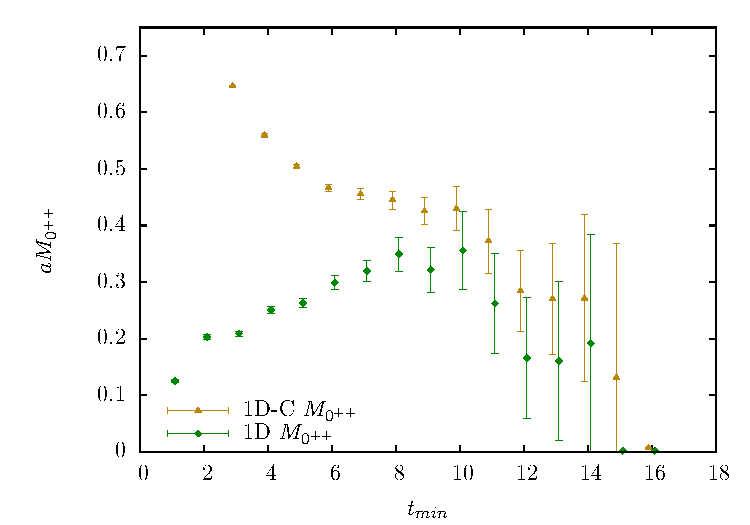
\includegraphics[width=2.5in]{./m0pp_zcen_cmp.pdf}\\
	\caption{Masses from non-linear fits from $t_{min}$ to the center of the correlator $N_t/2$.}
\end{figure}
\columnbreak
\begin{figure}[H]
\centering
    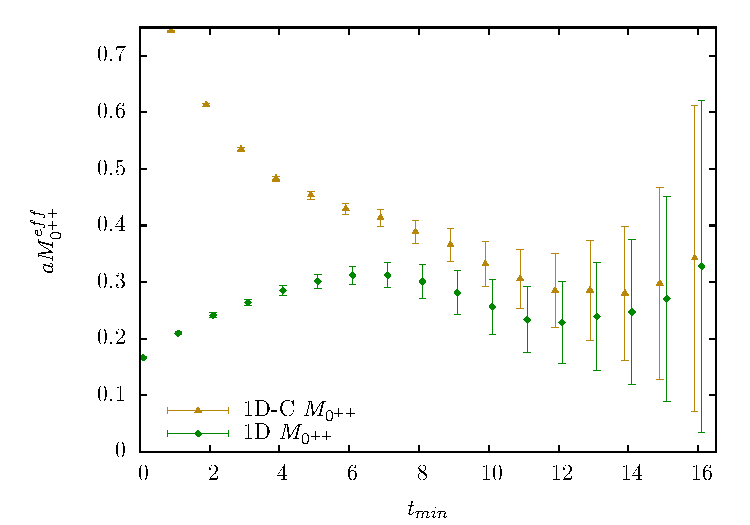
\includegraphics[width=2.5in]{./m0pp_zcen_eff.pdf}\\
	\caption{Kuti-style effective mass plots. }
\end{figure}
\end{multicols}

\begin{multicols}{2}
	\begin{figure}[H]
\centering
        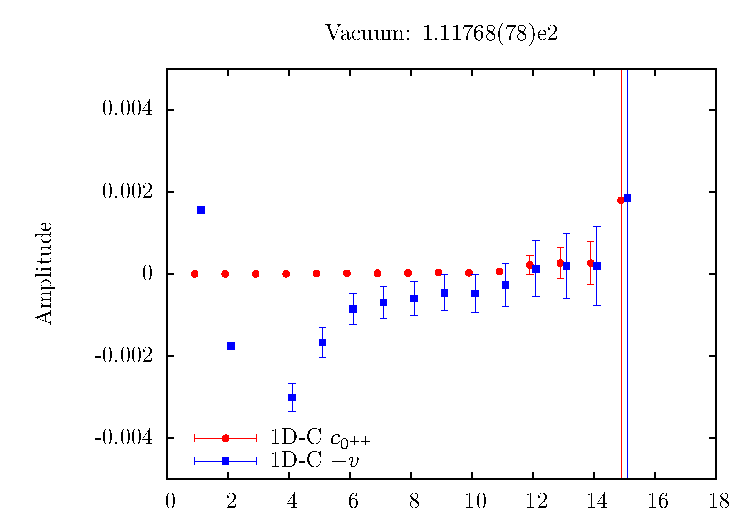
\includegraphics[width=2.5in]{./m0pp_zcen_amp.pdf}\\
	\caption{Amplitude and vacuum comparison (%NF%D-C) from non-linear fits from $t_{min}$ to the center of the correlator $N_t/2$.}
\end{figure}
\columnbreak
\begin{figure}[H]
\centering
    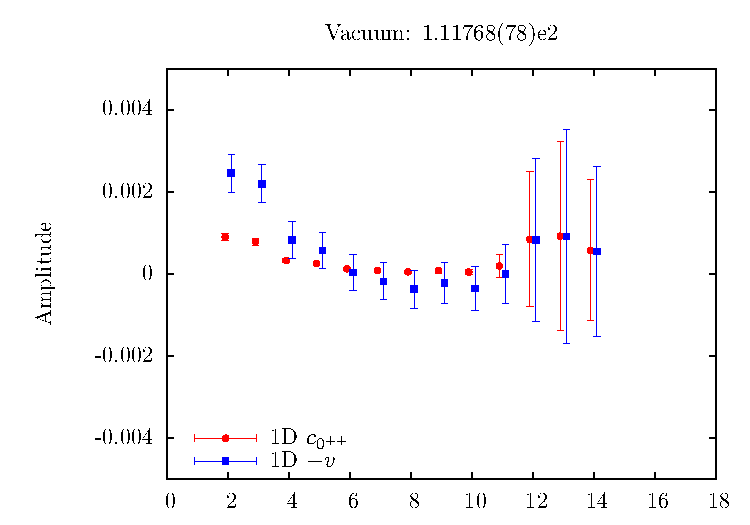
\includegraphics[width=2.5in]{./m0pp_zcen_amp_dc.pdf}\\
	\caption{Amplitude and vacuum comparison (%NF%D) from non-linear fits from $t_{min}$ to the center of the correlator $N_t/2$.}
\end{figure}
\end{multicols}

\begin{multicols}{2}
	\begin{figure}[H]
\centering
        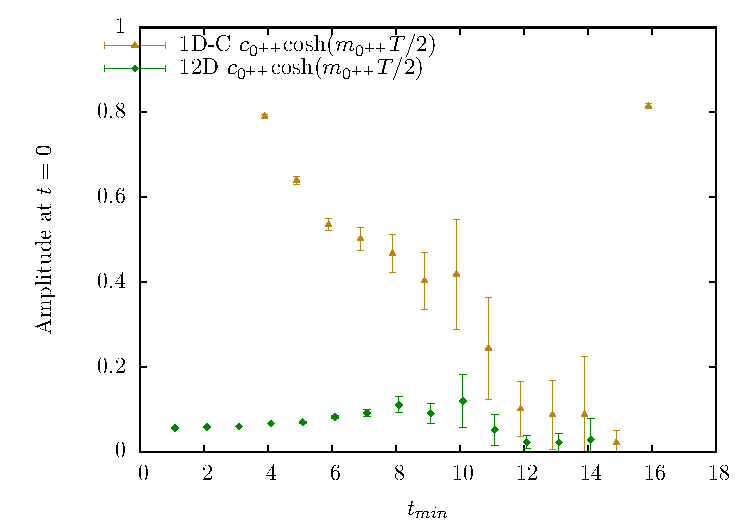
\includegraphics[width=2.5in]{./m0pp_zcen_amp_orig.pdf}\\
	\caption{Amplitude (propagated back to $t=0$) from non-linear fits from $t_{min}$ to the center of the correlator $N_t/2$.}
\end{figure}
\columnbreak
\begin{figure}[H]
\centering
        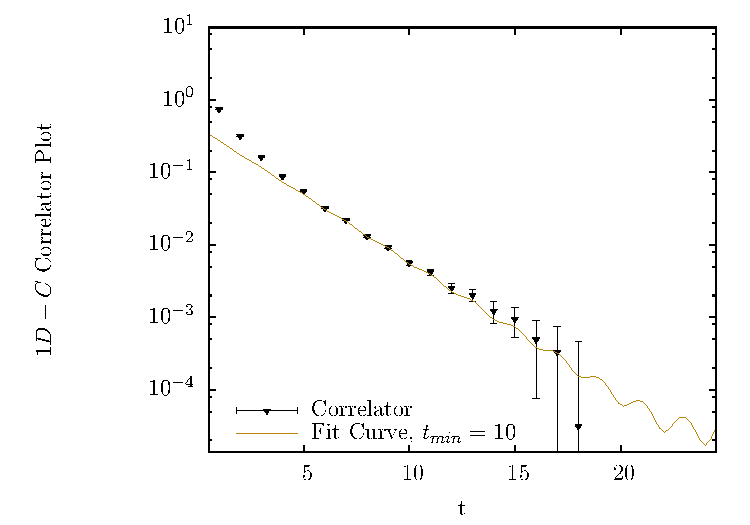
\includegraphics[width=2.5in]{./m0pp_zcen_fitlines.pdf}\\
        \caption{A sample fit of the data to a fit form. We look at %CORRNAME% using results from $t_{min} = %CORRTMIN%$.}
\end{figure}
\end{multicols}


\end{document}
